Hence, for a fixed $i_2$, the conditional distribution $\PP(X_1|X_2=i_2)\propto\begin{tikzpicture}[baseline=\baseline]
    \tikzset{tensor/.style = {minimum size = 0.5cm,shape = circle,thick,draw=black,inner sep = 0pt}, edge/.style = {thick,line width=.4mm},every loop/.style={}}
    \def\y{0.25}
    \def\x{0}
    \node[tensor,fill=blue!20!white] (T) at (\x,\y) {$\Tt$};
    \draw  node[fill = black,circle,inner sep=0pt,minimum size=4pt] (m_1) at (\x+0.5,\y-0.65) {};
    \draw[edge] (T) -- (\x-0.5,\y-0.65);
    \draw[edge](T) -- (\x,\y-0.75)node [very near end,below]
    {\scalebox{0.7}{\indcolor{$i_2$}}};
    \draw[edge](T) -- (m_1);
\end{tikzpicture}.$
\item We have $\PP(i_3|i_1,i_2) = \frac{\PP(i_1,i_2,i_3)}{\PP(i_1,i_2)}=\frac{\PP(i_1,i_2,i_3)}{\sum_{i_3}\PP(i_1,i_2,i_3)}
=
\frac{\begin{tikzpicture}[baseline=\baseline]
    \tikzset{tensor/.style = {minimum size = 0.5cm,shape = circle,thick,draw=black,inner sep = 0pt}, edge/.style = {thick,line width=.4mm},every loop/.style={}}
    \def\x{0}
    \def\y{0}
    \node[tensor,fill=blue!20!white] (T) at (\x,\y) {$\Tt$};
    \draw[edge] (T) -- (\x-0.5,\y-0.65)node [very near end,below]
    {\scalebox{0.7}{\indcolor{$i_1$}}};
    \draw[edge](T) -- (\x,\y-0.75)node [very near end,below]
    {\scalebox{0.7}{\indcolor{$i_2$}}};
    \draw[edge](T) -- (\x+0.5,\y-0.65)node [very near end,below]
    {\scalebox{0.7}{\indcolor{$i_3$}}};
\end{tikzpicture}}{\begin{tikzpicture}[baseline=\baseline]
    \tikzset{tensor/.style = {minimum size = 0.5cm,shape = circle,thick,draw=black,inner sep = 0pt}, edge/.style = {thick,line width=.4mm},every loop/.style={}}
    \def\x{0}
    \def\y{0}
    \node[tensor,fill=blue!20!white] (T) at (\x,\y) {$\Tt$};
    \draw  node[fill = black,circle,inner sep=0pt,minimum size=4pt] (m_2) at (\x+0.5,\y-0.65) {};
    \draw[edge] (T) -- (\x-0.5,\y-0.65)node [very near end,below]
    {\scalebox{0.7}{\indcolor{$i_1$}}};
    \draw[edge](T) -- (m_2);
    \draw[edge](T) -- (\x,\y-0.75)node [very near end,below]
    {\scalebox{0.7}{\indcolor{$i_2$}}};
\end{tikzpicture}},
$
for all $i_1, i_2$ and $i_3$.

Hence, for fixed $i_1$ and $ i_2$, the conditional distribution $\PP(X_3|X_1=i_1, X_2 = i_2)\propto\begin{tikzpicture}[baseline=\baseline]
    \tikzset{tensor/.style = {minimum size = 0.5cm,shape = circle,thick,draw=black,inner sep = 0pt}, edge/.style = {thick,line width=.4mm},every loop/.style={}}
    \def\y{0.25}
    \def\x{0}
    \node[tensor,fill=blue!20!white] (T) at (\x,\y) {$\Tt$};
    \draw[edge] (T) -- (\x-0.5,\y-0.65)node [very near end,below]
    {\scalebox{0.7}{\indcolor{$i_1$}}};
    \draw[edge](T) -- (\x,\y-0.75)node [very near end,below]
    {\scalebox{0.7}{\indcolor{$i_2$}}};
    \draw[edge](T) -- (\x+0.5,\y-0.65);
\end{tikzpicture}.$ 
\end{enumerate}
\subsubsection{Tensor Train Parameterization of Probability Distributions}
As we saw in Section~\ref{chapter:tensor-decomposition}, working with high-order tensors becomes computationally expensive because the number of elements grows exponentially with the tensor order. This also applies to tensors representing joint probability distributions: the tensor representation grows exponentially with the number of random variables. One way to address this issue is to parameterize the probability tensor as a low-rank tensor network.

We will show here how this can be done with the tensor train decomposition. This can also be done with other decomposition models, but the tensor train format is particularly interesting and has been used very successfully in quantum physics to model many-body systems~\citep{TensorNetworkOrg}.

Let $\Tt\in\RR^{d_1\times\cdots\times d_N}$ be a probability tensor parameterized in the tensor train format: 
\begin{center}
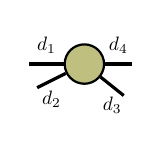
\begin{tikzpicture}[baseline=-0.5ex]
    \tikzset{tensor/.style = {minimum size = 0.5cm,shape = circle,thick,draw=black,inner sep = 0pt}, edge/.style = {thick,line width=.4mm},every loop/.style={}}
    \def\x{6}
    \def\y{0}
     \node[tensor,fill=green!50!red!50!white] (B) at (\x+1,\y) {$\Tt$};
    \draw[edge] (B) -- (\x+0.3,0) node [midway,above] {\scalebox{0.7}{\dimcolor{$d_1$}}};
    \draw[edge] (B) -- (\x+1.6,0) node [midway,above] {\scalebox{0.7}{\dimcolor{$d_4$}}};
    \draw[edge] (B) -- (\x+0.4,-0.3) node [midway, below] {\scalebox{0.7}{\dimcolor{$d_2$}}};
    \draw[edge] (B) -- (\x+1.5,-0.4)node [midway, below] {\scalebox{0.7}{\dimcolor{$d_3$}}};
\end{tikzpicture}
=
\begin{tikzpicture}[baseline=\baseline]
    \tikzset{tensor/.style = {minimum size = 0.5cm,shape = circle,thick,draw=black,inner sep = 0pt}, edge/.style   = {thick,line width=.4mm},every loop/.style={}}
    \def\y{0}
    \def\x{0}
  \node[tensor,fill=red!30!white] (D) at (\x-1,\y){$\Gt_1$};
  \node[tensor,fill=red!50!white] (A) at (\x,\y){\scalebox{0.85}{$\Gt_2$}};
  \node[tensor,fill=blue!50!white] (B) at (\x+1,\y){$\Gt_3$};
   \node[tensor,fill=blue!20!white] (C) at (\x+2,\y){$\Gt_4$};
    \draw[edge](A) -- (\x,\y-0.7)node [midway,left] {\edgelabel{$d_2$}};
    \draw[edge](B) -- (\x+1,\y-0.7)node [midway,left] {\edgelabel{$d_3$}};
    \draw[edge](C) -- (\x+2,\y-0.7)node [midway,left] {\edgelabel{$d_4$}};
     \draw[edge](D) -- (\x-1,\y-0.7)node [midway,left] {\edgelabel{$d_1$}};
    \draw[edge](D) -- (A) node [midway,above] {\edgelabel{$R_1$}};
    \draw[edge](A) -- (B) node [midway,above] {\edgelabel{$R_2$}};
    \draw[edge](B) -- (C) node [midway,above] {\edgelabel{$R_3$}};
\end{tikzpicture}.
\end{center}

Since $\Tt$ represents a probability distribution, its entries must be non-negative and sum to one.
In the context of machine learning, where we want to optimize the core tensors with respect to some loss function~(e.g. log-likelihood), there are several constraints one can impose on the core tensors $\Gt_1,\cdots,\Gt_N$ to ensure these two properties. 
One easy way to ensure non-negativity of the entries of $\Tt$ is to constrain the core tensors to have non-negative entries, or to apply a non-negative valued "activation" function component-wise to all the core tensors' entries. Another way, with its roots in quantum physics, is to assume that the entries of $\Tt$ are the square roots of the probabilities, rather than the probabilities themselves: $\Tt_{i_1,\cdots,i_N} = \sqrt{\PP(X_1=i_1,\cdots,X_N=i_N)}$. When $\Tt$ is in the TT format, this corresponds to the following tensor network:
$$
\PP(X_1=i_1,\cdots,X_4=i_4) = (\Tt_{i_1,\cdots,i_4})^2 = 
\begin{tikzpicture}[baseline=\baseline]
    \tikzset{tensor/.style = {minimum size = 0.5cm,shape = circle,thick,draw=black,inner sep = 0pt}, edge/.style   = {thick,line width=.4mm},every loop/.style={}}
    \def\y{-0.35}
    \def\x{0}
  \node[tensor,fill=red!30!white] (D) at (\x-1,\y){$\Gt_1$};
  \node[tensor,fill=red!50!white] (A) at (\x,\y){\scalebox{0.85}{$\Gt_2$}};
  \node[tensor,fill=blue!50!white] (B) at (\x+1,\y){$\Gt_3$};
   \node[tensor,fill=blue!20!white] (C) at (\x+2,\y){$\Gt_4$};
   \node[tensor,fill=red!30!white] (G1) at (\x-1,\y+0.85){$\Gt_1$};
  \node[tensor,fill=red!50!white] (G2) at (\x,\y+0.85){\scalebox{0.85}{$\Gt_2$}};
  \node[tensor,fill=blue!50!white] (G3) at (\x+1,\y+0.85){$\Gt_3$};
   \node[tensor,fill=blue!20!white] (G4) at (\x+2,\y+0.85){$\Gt_4$};
    \draw[edge](G1) -- (\x-1,\y+1.65)node [very near end, above]{\scalebox{0.7} {\indcolor{$i_1$}}};
    \draw[edge](G2) -- (\x,\y+1.65)node [very near end, above]{\scalebox{0.7} {\indcolor{$i_2$}}};
    \draw[edge](G3) -- (\x+1,\y+1.65)node [very near end, above]{\scalebox{0.7}{\indcolor{$i_3$}}};
    \draw[edge](G4) -- (\x+2,\y+1.65)node [very near end, above]{\scalebox{0.7}{\indcolor{$i_4$}}};
    \draw[edge](G1) -- (G2)node [midway,above] {\edgelabel{$R_1$}};
    \draw[edge](G2) -- (G3)node [midway,above] {\edgelabel{$R_2$}};
    \draw[edge](G3) -- (G4)node [midway,above] {\edgelabel{$R_3$}};
    \draw[edge](A) -- (\x,\y-0.7)node [very near end, below] {\scalebox{0.7}{\indcolor{$i_2$}}};
    \draw[edge](B) -- (\x+1,\y-0.7)node [very near end, below]{\scalebox{0.7} {\indcolor{$i_3$}}};
    \draw[edge](C) -- (\x+2,\y-0.7)node [very near end, below] {\scalebox{0.7}{\indcolor{$i_4$}}};
     \draw[edge](D) -- (\x-1,\y-0.7)node [very near end, below] {\scalebox{0.7}{\indcolor{$i_1$}}};
    \draw[edge](D) -- (A) node [midway,above] {\edgelabel{$R_1$}};
    \draw[edge](A) -- (B) node [midway,above] {\edgelabel{$R_2$}};
    \draw[edge](B) -- (C) node [midway,above] {\edgelabel{$R_3$}};
\end{tikzpicture}
.
$$

